\chapter{Theoretical Background}
\label{chap:theory}

Evolving over the course of decades of theoretical insights and
experimental discoveries, the Standard Model (SM) of particle physics
can be viewed as a success of the scientific method. In its current
incarnation, the SM describes three of the four elementary particle
interactions, predicting with surprising accuracy the spectrum of
these particles and the strengths with which they interact. These
predictions-- governing interactions within dying stars, nuclear
reactors, and in the universe immediately after its birth--- are
derived from fundamental symmetries known to exist in nature. In this
chapter, the theoretical framework for the Higgs boson measurement
presented in this thesis is laid out, starting with a description of
the SM. From there, an application of the SM to physics in hadron
colliders is discussed, and the chapter
concludes with a look at the nature of the Higgs boson at the Large
Hadron Collider. 

\section{The Standard Model}
\label{chapter:theory:section:sm_intro}

The SM seeks to predict the spectrum of, and
interactions among, the particles that constitute matter. Since these
elementary particles are infinitesimally small, their behavior is
governed by the postulates of quantum mechanics (QM). More
specifically, the SM is built on a theoretical framework known as
quantum field theory (QFT), a relativistic extension of classical
QM. QFT improves on classical QM by allowing particle number
to be violated in a closed system, a phenomenon that is observed in,
for example, an atomic energy level transition whereby a photon is
created or annihiliated. Particles in QFT are described as excited states
of space-time fields that are realized as mathematical
operators. These operators serve to create or annihilate particles. The
dynamics of a field, and its associated
particles, is obtained from a Lagrangian density,
$\mathcal{L}(\phi,\partial_{\mu}\phi)$, the field-theoretic
analogue of the Lagrangian in classical mechanics. In the context of
QFT, if two different fields appear in the same term of $\mathcal{L}$, the two
particles associated with these fields are said to ``couple''. It is
these couplings that lead to the fundamental interactions. 

Elementary particles broadly fall into two categories: half-integer
spin fermions and integer spin bosons. Quarks and leptons, for example, are fermions
with spin-1/2, while the particle that mediates the electromagnetic
(EM) interaction, the photon, is a spin-1 boson. Dirac formulated a
relativistic analogue of the Schrodinger equation for spin-1/2
particles, and the corresponding Lagrangian is

\begin{equation}
\mathcal{L}_{\textrm{fermion}} =
i\bar{\psi}\gamma_{\mu}\partial^{\mu}\psi - m\bar{\psi}\psi.
\label{chap:theory:equation:dirac_lagrangian}
\end{equation}

\noindent
To incorporate the two spin states of the fermion and the
fact that each particle has an antiparticle, the field $\psi$ has four
degrees of freedom. In the above equation, $\bar{\psi} =
\psi^{\dagger}\gamma^0$, where $\psi^{\dagger}$ denotes the
adjoint. The $\gamma^{\mu}$ are the Dirac $\gamma$-matrices,
whose anticommutators form the Dirac algebra:
$\left\{\gamma^{\mu},\gamma^{\nu}\right\} = 2g^{\mu\nu}$. The first term
of equation~\ref{chap:theory:equation:dirac_lagrangian} is the kinetic
energy term, and the second is the mass term that gives a mass $m$ to
the particle associated with the field. 

Particles that are excitations of the fields described by
equation~\ref{chap:theory:equation:dirac_lagrangian} do not interact
with eachother, which is empirically known to be false. Charged
electrons experience an electromagnetic force from the atomic nucleus,
whose constituents are bound together by the strong interaction. Some
of these nuclei emit radiation as a consequence of the weak interaction. In the
SM, these three forces are incorporated as additional terms in
$\mathcal{L}_{\textrm{fermion}}$. The fourth fundamental interaction,
gravity, has not been successfully included in the model. Inter-field
interactions arise when a local gauge symmetry is imposed. These
so-called symmetries are in fact just internal mathematical degrees of
freedom that are not expected to impact the observed behavior of a field. For
example, the local phase of a field, $\alpha(x)$, does not correspond
to a physical quantity. Therefore, the Lagrangian should be
invariant under the transformation $\psi\rightarrow
e^{-ig\alpha(x)}\psi$. The non-interacting Lagrangian
in equation~\ref{chap:theory:equation:dirac_lagrangian} does not fulfill this
requirement. However, if a new field is introduced through a
term of the form $g\bar{\psi}\gamma^{\mu}\psi A_{\mu}$,
$\mathcal{L}_{\textrm{fermion}}$ becomes invariant as long as the new
field transforms as $A_{\mu}\rightarrow{A_{\mu}
+ \partial_{\mu}\alpha(x)}$. The vector field
$A_{\mu}$ is called a gauge field, and it represents the photon. 
Because this new field represents a
physical particle, a kinetic energy term associated with $A_{\mu}$
needs to be introduced. A choice that preserves gauge and Lorentz
invariance is a kinetic energy term of the form $-(1/4)F_{\mu\nu}F^{\mu\nu}$,
where $F_{\mu\nu}$ is the EM field strength tensor. A mass term for $A_{\mu}$ is not included in the
Lagrangian, because it breaks gauge invariance. The photon, therefore,
is considered to be massless. It can be shown
that a Lagrangian of this form for $A_{\mu}$ recovers Maxwell's
equations.

An important property of the gauge transformation
$e^{-ig\alpha(x)}$ is that it forms a Lie group under
multiplication~\cite{}. In general, any element of a Lie group can be
written as $e^{-i\alpha_j(x)X_j}$, where the $X_j$ are the group
generators and the parameters $\alpha_j(x)$ identify each element of the
group. For a gauge theory, the number of generators is equal to the
number of gauge fields that arise when invariance is imposed in the
Lagrangian. Furthermore, the nature of the resulting gauge interactions is defined
by the commutation relations among the generators:
$\left[X_i,X_j\right] = if_{ijk}X_k$, where the $f_{ijk}$ are real
constants called the structure constants.

For the EM interaction, the symmetry group is $U(1)$, an Abelian group which
has a single generator, which, as discussed above, results in the photon. For the weak
interaction, the internal symmetry is weak isospin, which is described by the Lie group
$SU(2)$. With three generators, $SU(2)$ gauge invariance produces three
fields associated with the weak vector bosons $W^+$, $W^-$, and
$Z$. In the theory of the strong interaction, called quantum chromodynamics
(QCD), an $SU(3)$ color symmetry is required, resulting in eight gauge
fields associated with gluons. Apart from producing more gauge fields,
the $SU(2)$ and $SU(3)$ symmetries differ from the $U(1)$ symmetry of
the EM interaction because they have non-zero
structure constants. A consequence of this differing group structure
is that self-interaction terms arise in the Lagrangian. Hence, both
gluons and weak vector bosons can couple to themselves. 

In EM, the inclusion of a mass term for $A_{\mu}$ breaks the $U(1)$
gauge symmetry. This is easily resolved by setting the mass of the
photon to zero. The same problem arises in both strong and weak
Lagrangians. In the case of QCD, the eight gluon masses are set to
zero, and color symmetry is restored. The masses of the three weak
gauge bosons, on the other hand, have been measured to be non-zero. In
fact, these particles are quite massive: $m_W = 80.4 \gev$ and $m_Z =
90.1 \gev$. If the gauge symmetry is broken by introducing mass
terms, infinities are induced in the perturbative
expansion of the path integral which can not be renormalized,
rendering the theory non-predictive. 

In addition to the weak
boson mass terms, the fermion mass terms
in the weak Lagrangian violate the $SU(2)$ symmetry. Since the weak
interaction has been measured to maximally violate the discrete
symmetry known as parity, gauge invariance is only required for
left-handed fields, though both left and right-handed fermion fields
exist in nature and hence, in the Lagrangian. With a mixture of
helicity states in the mass term, each transforming differently under
$SU(2)$, the symmetry is broken. The prediction implied by setting all
fermion masses to zero is at odds with a myriad of experimental
evidence. These theoretical problems with the weak boson and fermion
masses led to the development of spontaneous symmetry breaking. 

An approach for simultaneously introducing both gauge boson and
fermion mass terms
into the Lagrangian, while preserving gauge symmetry and
renormalizability, was developed in the 1960s~\cite{}, and was
subsequently adapted for the unified electroweak theory~\cite{}. A
complex scalar field that transforms as a weak isospin doublet, and is
described by the Lagrangian

\begin{equation}
\mathcal{L}_{\textrm{Higgs}} =
\left(D_{\mu}\phi^{\dagger}\right)\left(D^{\mu}\phi\right)
- \left[ \mu^2 \phi^{\dagger}\phi + \lambda (\phi^{\dagger}\phi)^2\right]
\label{chap:theory:equation:higgs_lagrangian}
\end{equation}

\noindent
is introduced into the Lagrangian describing both EM and weak
interactions. This form is chosen to be invariant under the gauge
symmetry $SU(2) \times U(1)$, and due to the restrictions $\mu^2 < 0$
and $\lambda > 0$, to yield non-zero $\phi$ at the potential energy
minimum. In the QFT context, the $\phi$ value that minimizes the
potential energy, denoted $\phi_0$, corresponds to the physical
absence of particle excitations associated with the field, and is
therefore known as the vacuum expectation value (vev). The manifold on
which the potential is minimized is, from the invariance of
$\mathcal{L}_{\textrm{Higgs}}$, manifestly invariant under
$SU(2) \times U(1)$. The $SU(2)$ symmetry is then broken ``spontaneously''
when a point on the manifold is chosen, or, equivalently, when a gauge
is chosen. This process is spontaneous in the sense that there is not
a dynamical theory for why it occurs; it is merely postulated that it
has occurred. 

By performing a gauge transformation on the resulting isospin doublet
$\phi_0$, the non-zero expectation value can be projected into the
real part of the neutral component of the doublet, leaving the three
remaining real scalar degrees of freedom with a magnitude of zero.
To recover the dynamics, the remaining scalar component is perturbed
about the vacuum expectation value--- $v + H(x)$--- where the field
$H(x)$ is a real scalar field known as the Higgs field. Putting this
expression for $\phi$ into
equation~\ref{chap:theory:equation:higgs_lagrangian}, mass terms for
$W^{\pm}$ and $Z$ are generated in the mixing of the $v$ part of the
field and bilinear gauge boson terms in the covariant derivative
$D_{\mu}$. Additional gauge invariant terms that mix $\phi$
and bilinear fermion terms are added to the Lagrangian, resulting in
mass terms when $\phi$ acquires a vev. This mechanism, therefore, is successful in mitigating the two
deficiencies outlined above. An important bi-product of this mechanism
for generating masses is the prediction of the existence of a spin-0
particle, hereafter referred to as the Higgs boson or the
Higgs. The Higgs boson couples to fermions and gauge bosons with a
strength proportional to their masses, implying that direct production of
such a particle is possible at colliders. Moreover, such couplings
induce higher order corrections in measureable quantities such as the
top quark and $W$ boson masses. Consequently, the existence of the
Higgs boson can be indirectly established by measuring deviations in
these observables. Though the
Lagrangian~\ref{chap:theory:equation:higgs_lagrangian} appears to
introduce two new parameters to the SM, one can be related to existing
SM input parameters, leaving only one parameter that can be expressed
in terms of the mass of the Higgs boson ($m_H$).

The above procedure, known popularly as the Higgs mechanism, restores the gauge
symmetry of the SM Lagrangian, thereby ensuring
renormalizability. The underlying $SU(2)$ symmetry of the weak
interaction is hidden, or spontaneously broken, resulting in a
tangible prediction, the existence of a massive, spin-0 boson whose
coupling to other particles is linear with their masses. Other scalar
degrees of freedom in the field $\phi$ become the longitudinal
polarization of the weak gauge bosons, a necessary property of massive
spin-1 particles. This form of the Higgs mechanism is not unique; the
chosen representation of $SU(2)$, namely that $\phi$ is a complex
scalar doublet, is merely the most parsimonious. Additional degrees of
freedom arise if another representation is chosen or if an additional
$SU(2)$ invariant Higgs fields are introduced. In some cases, these
extended Higgs scenarios, which predict additional Higgs particles,
fix other theoretical limitations of the SM. However, because every
incarnation of the Higgs mechanism has at least one neutral scalar Higgs boson,
the minimalistic form is chosen in the SM. 

In its current form, the SM is a gauge theory obeying $SU(3) \times
SU(2) \times U(1)$ symmetry, resulting in a total of 12 gauge bosons:
8 massless, bi-colored gluons, 3 massive weak vector bosons, and a
single massless photon. Three fermion generations, each with a charged
lepton, a neutrino, two quarks, as well as their corresponding
anti-matter particles, have been observed, totaling 48
fermions. Adding to the list the all-important Higgs boson, 61
particles are predicted to exist by the SM, all of which have been
experimentally observed. 





%\section{Triumphs of the SM}
%\input{tex/theory/sm_triumphs}

\section{The SM at hadron colliders}
\label{chapter:theory:section:collider_physics}

Starting with Rutherford's gold foil experiment, scattering
experiments that measure the deflection of particles in the presence
of some form of matter have been effective in probing the structure of
matter and the forces with which it interacts. Such experiments have
proved to be invaluable testing grounds for the SM. The gauge
structure of the SM has historically been tested by either looking for
evidence of particles introduced in the process of enforcing gauge
symmetry, if those particles had not yet been observed, or if they
had, by measuring the degree to which gauge bosons couple to
fermions and themselves. The coupling strength between fields is
related to a quantity called the cross section which is a measure of
the probability with which a scattering process occurs. For the
scattering of two particles into $n$ particles, the cross section can
be written

\begin{equation}
\hat{\sigma}_{qq\rightarrow{n}} = \int_{\mathscr{V}_n} |M(q_1,q_2;y_1,...,y_n)|^2
d\Phi_n(q_1+q_2;y_1,...,y_n)
\label{chapter:theory:equation:cross_section}
\end{equation}

\noindent
where the $q_i$ ($y_i$) are the momentum 4-vectors of the incoming
(outgoing) particles. The differential $d\Phi_n(q_1+q_2;y_1,...,y_n)$ is the Lorentz
invariant phase space term that enforces conservation of energy and
momentum, and $M(q_1,q_2;y_1,...,y_n)$ is the matrix element that
captures the dynamics of the Lagrangian. It is calculated with the
perturbative techniques of QFT. Therefore, measuring the cross
section $\hat{\sigma}$ for a given scattering process is an effective
test of the relevant terms in the Lagrangian. 

\begin{figure}[h]
\centering
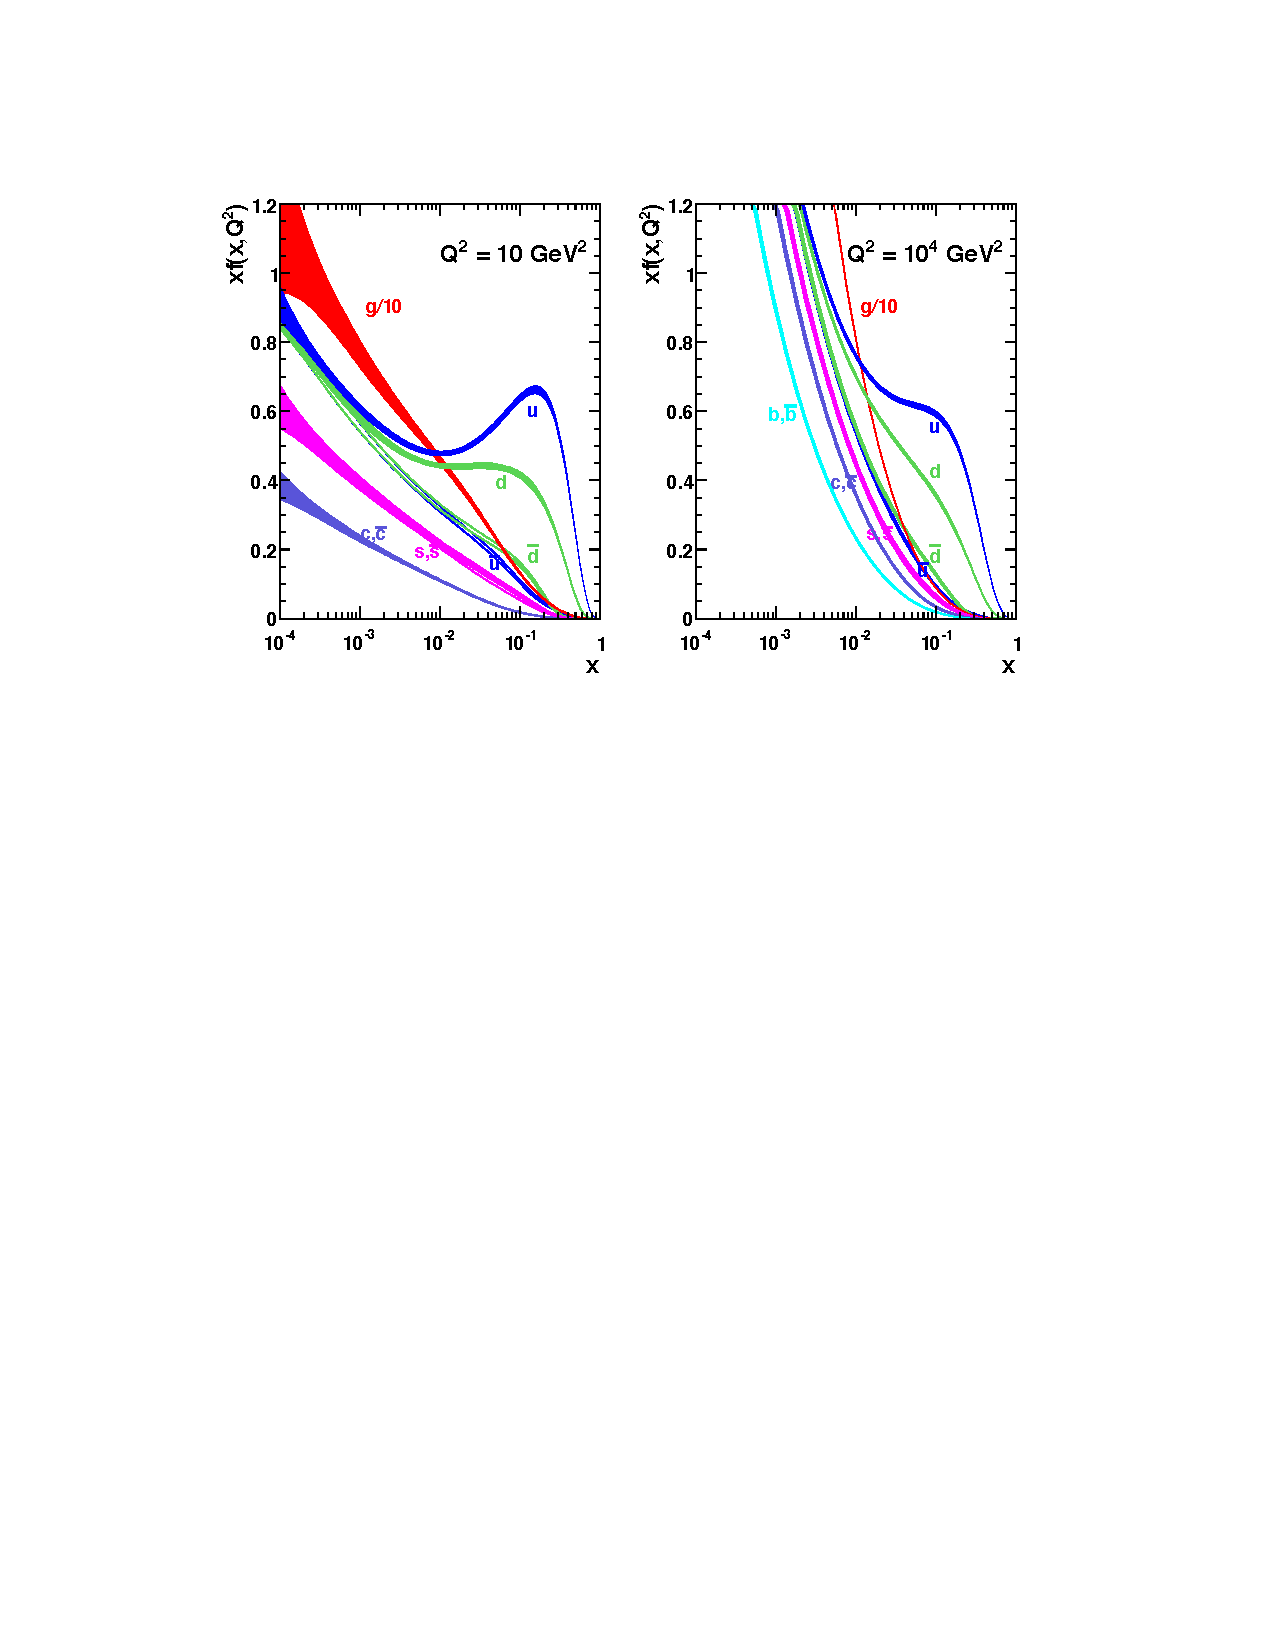
\includegraphics[width=1.0\textwidth]{fig/theory/mstw_pdfs.pdf}
\caption{\cite{bib:Martin:2009iq}}
\label{chap:theory:fig:pdf_set}
\end{figure}

The expression for $\sigma$ defined in
equation~\ref{chapter:theory:equation:cross_section} applies to the
scattering of two elementary particles into $n$ particles. At the LHC,
the two incident particles are protons, which are composite particles
composed of quarks interacting through gluon exchange. Due to the
non-Abelian structure of the gauge group governing these interactions,
as well as the fact that gluons are massless, quarks and gluons can be
described as free particles at sufficiently high energy scales. This
phenomenon, a consequence of the fact that the strong coupling
constant decreases with increasing energy scales, is called
``asymptotic freedom''. It allows the perturbation techniques of QFT
to be used for QCD predictions at energy scales above
$\Lambda_{\textrm{QCD}}$. Below this scale, heuristic non-perturbative
models are used. Particles that are composed of quarks, such as
protons, must have a configuration of two or three quarks that
transforms as an $SU(3)$ color singlet. Protons are composed of three
valence quarks--- two up quarks and a down quark--- as well as a
``sea'' of gluons and quarks of other flavors due to excitations
between the valence quarks. Parton distribution functions (pdfs)
quantify the probability that a given parton within the proton carries
a momentum fraction $x$ of the total proton momentum. These pdfs have
been determined as a function of the energy scale at
which the proton is probed through a global fit of data from deep inelastic scattering (DIS) and
other high energy collider experiments~\cite{bib:Martin:2009iq}. In
figure~\ref{chap:theory:fig:pdf_set}, the results of these fits are
shown as the product of the parton momentum fraction and the pdf,
$xf(x,Q^2)$, which represents the momentum density for a given
parton. At high $x$, the valence quarks carry the majority of the
momentum, and at low $x$ the sea partons begin to contribute momentum,
with the gluon pdf dramatically larger than the others (note that the
gluon distribution is scaled down by a factor of 10). This behavior
turns out to be important in Higgs physics at the LHC
(section~\ref{chapter:theory:section:higgs_physics}).

For proton-proton scattering, the cross section
is computed by weighting the quark-quark scattering cross
sections (e.g. equation~\ref{chapter:theory:equation:cross_section})
by the pdfs and integrating over the momentum fractions:

\begin{equation}
\sigma_{pp\rightarrow{n}} = \int dx_1 dx_2 f_{q_1}(x_1,\mu_F)
  f_{q_2}(x_2,\mu_F) \hat{\sigma}_{qq\rightarrow{n}}.
\label{chapter:theory:equation:cross_section_pp}
\end{equation}

\noindent
Here, $f_{q_1}$ ($f_{q_2}$) is the pdf for a quark of
flavor $q_1$ ($q_2$) and momentum fraction $x_1$ ($x_2$). The cross
section is now expressed in terms of the perturbative cross section
associated with the free partons, with the non-perturbative part
factorized into the pdfs. The scale that separates the two regimes is
called the factorization scale, $\mu_F$. As more terms are included in
the perturbative expansion of $\hat{\sigma}_{qq\rightarrow{n}}$,
divergences arise when, for example, QCD radiation is soft or
collinear. To make the theory predictive again,
$\hat{\sigma}_{qq\rightarrow{n}}$ is renormalized at some scale
$\mu_R$. The resulting cross section calculated at all orders in
perturbation theory is invariant with respect to changes in $\mu_F$
and $\mu_R$. However, due to calculational difficulties, the cross
section is computed at fixed order in perturbation theory,
making it necessary to vary $\mu_F$ and $\mu_R$, and quantify the
change in the predicted cross section. This change is then assigned as
an experimental uncertainty. 

In most scattering experiments, a prediction is obtained from Monte
Carlo (MC) simulation, whereby an event is generated probabilistically
by drawing from the differential cross section distribution defined
by~\ref{chapter:theory:equation:cross_section_pp}. MC generators are
able to generate a hard scattering up to some fixed order, and to augment
fixed order calculations, parton shower (PS) programs are typically
interfaced to the MC generator, allowing diagrams with more vertices
to be modeled. For a quark or gluon in the final state, the PS program
uses the DGLAP equation~\cite{} to model the emission of additional
quarks and gluons down to some cut-off energy scale in a process known
as fragmentation. The resulting partons, which are not confined to color
singlet configurations, are then hadronized using a non-perturbative
model, forming a collection of hadrons that are observable to the
detector. The shower of hadrons associated with a final state quark or
gluon is known as a jet (discussed in more detail in
chapter~\ref{chapter:reconstruction}).

In the electroweak sector of the SM, the gauge structure is tested by
measuring evidence for diagrams that only arise when gauge
invariance is imposed, and by comparing the cross sections of such
processes to the SM predictions. The LHC, with its high
center-of-mass energy, is sensitive to many of these processes, as
shown in figure~\ref{chap:theory:fig:xs_summary_plot}, which
summarizes the cross sections measured by the ATLAS detector for some
important SM processes. The production of a single $W$ or $Z$ boson is
precisely measured to be consistent with the SM prediction. Processes
involving the production of two weak gauge bosons--- $WW$, $WZ$, and
$ZZ$--- are also in agreement with the SM. Such self-consistent
predictions provide strong evidence for the gauge structure of the
SM. 

\begin{figure}
\centering
\includegraphics[width=1.0\textwidth]{fig/theory/ATLAS_c_SMSummary_TotalXsect_rotated.eps}
\caption{}
\label{chap:theory:fig:xs_summary_plot}
\end{figure} 



\section{Higgs physics at the LHC}
\label{chapter:theory:section:higgs_physics}

Prior to the summer of 2012, the gauge structure of the SM had held up
to repeated experimental tests, with the exception of one crucial
part--- evidence of the Higgs boson associated with $SU(2) \times
U(1)$ symmetry breaking. This long sought after particle had been one
of the primary motivations for the construction of the LHC, a $pp$
collider with a center-of-mass energy (\sqrts) expected to be large
enough to observe the particle. Following the discovery of the Higgs
boson in July 2012, LHC experiments entered a new phase of precision
measurements of the Higgs couplings. In the following section, Higgs
physics at the LHC is discussed.

The introduction of the Higgs field into the SM Lagrangian gives rise
to a consistent set of testable predictions. The Higgs boson should
behave like a chargeless spin-0 particle. It should couple to weak
gauge bosons through terms of the form $HVV$ ($V=W/Z$), with a strength
proportional to the square of the mass of the gauge boson. Moreover, as a
consequence of fermion mass generation, the Higgs boson should couple
to fermions with a strength that grows linearly their masses. Because the
masses of the gauge bosons and fermions are well-measured, the Higgs
couplings are determined. In fact, the only remaining parameter to which
Higgs predictions are sensitive is the mass of the Higgs boson $m_H$,
which is not constrained by the theory itself. It is, however,
argued that, if the theory is to remain unitary and have a stable vacuum,
the Higgs mass should lie in the range $50 \gev \lesssim m_H \lesssim
800 \gev$~\cite{bib:Djouadi:2005gi}. Since the Higgs boson is a
massive particle that couples to both fermions and gauge bosons, it is
found in loop diagrams at higher orders in perturbation theory. These
diagrams contribute non-negligible corrections to SM input parameters
that are observable in precision electroweak measurements. Using such measurements
from the LEP, SLC, and Tevatron experiments, $m_H$ had been
constrained to be $91^{+30}_{-23} \gev$ at the one standard deviation
level prior to the discovery~\cite{bib:Baak:2011ze}. \note{Show $\chi^2$
figure?}. A direct search done at LEP2 placed a lower bound of $m_H >
114.4 \gev$ at the 95\% confidence level. These experimental
constraints helped to guide the LHC experiments prior to the Higgs
discovery. Following the discovery, the Higgs mass has been measured
to be $125.7 \pm 0.4$ by the CMS collaboration~\cite{bib:CMS-PAS-HIG-13-005} and $125.36 \pm
0.41$ by the ATLAS collaboration~\cite{bib:Aad:2014aba}. 

\begin{figure}[h]
    \centering
    \subfigure[ggF]{
    \includegraphics[width=0.45\textwidth]{fig/theory/ggf_diag.pdf}
    \label{chap:theory:fig:higgs_diag_ggf}
    }
    \subfigure[VBF]{
    \includegraphics[width=0.40\textwidth]{fig/theory/vbf_diag.pdf}
    \label{chap:theory:fig:higgs_diag_vbf}
    }
    \subfigure[$VH$]{
    \includegraphics[width=0.45\textwidth]{fig/theory/vh_diag.pdf}
    \label{chap:theory:fig:higgs_diag_vh}
    }
    \subfigure[$t\bar{t}H$]{
    \includegraphics[width=0.40\textwidth]{fig/theory/tth_diag.pdf}
    \label{chap:theory:fig:higgs_diag_tth}
    }
    \caption[]{}
\label{chap:theory:fig:higgs_diagrams}
\end{figure}

The dominant mechanisms for the production of a Higgs boson at
a $pp$ collider, shown in terms of Feynman diagrams in
figure~\ref{chap:theory:fig:higgs_diagrams}, are dictated by the fact
that the Higgs boson preferentially couples to more massive particles. The
process with the
largest cross section is gluon-gluon fusion (ggF), $gg\rightarrow{H}$, characterized by
two incoming gluons that effectively couple to the Higgs through a
quark loop. Only the heavy top and bottom quarks contribute in this loop. If the
center-of-mass energy is large with respect to $m_H$, then the Higgs
can be produced with a small fraction of the incoming proton
momentum, or in the $x$ region where the gluon pdf is
large (figure~\ref{chap:theory:fig:pdf_set}). Higgs production by direct coupling between the Higgs
and incoming quarks is suppressed by the pdfs for the heavy quarks for
which there is a non-negligible coupling to the Higgs.

The second largest Higgs production mechanism at $pp$ colliders is the
vector boson fusion (VBF) process, whereby two incoming quarks radiate
virtual weak gauge bosons that then fuse to form the Higgs,
$qq\rightarrow{q^{\prime}q^{\prime}V^{\ast}V^{\ast}}\rightarrow{q^{\prime}q^{\prime}H}$. Though
this process can proceed via either $W$ or $Z$ fusion, the
contribution of the $W$ diagram is around three times that of the $Z$,
due to the fact that $W$ bosons couple more strongly to
fermions~\cite{bib:Djouadi:2005gi}. In spite of the smaller cross
section, this process is a powerful probe of the Higgs sector due to its
characteristic final state. Since the energy of the radiated weak
bosons is significantly less than that of the incoming quarks, the
deflection of these quarks is small, and therefore the outgoing quarks
manifest as high energy forward jets. Another feature of these events is that
there is little QCD radiation between the outgoing quarks, due to the
absence of the flow of color between them. These two characteristics
allow such Higgs events to be efficiently isolated from the background
events, which, in hadron colliders, are likely to include central
jets. 

Associated production of the Higgs with either weak gauge bosons or
top quarks is also visible at the LHC. The former occurs when the initial state quarks form an
off-shell gauge boson that then splits into a Higgs and a gauge boson:
$qq\rightarrow{V^{\ast}\rightarrow{VH}}$. The latter process is
similar to ggF in that an effective coupling between gluons and the
Higgs is mediated through top quarks, but in this case the quarks
appear as outgoing particles: $gg\rightarrow{t\bar{t}H}$. 

\begin{table}
\begin{center}
\renewcommand{\arraystretch}{1.2}
%\resizebox{0.8\textwidth}{!}{
    \begin{tabular}{ l | c }
    \hline
    Higgs Decay & Branching Fraction \\
    \hline \hline
    $b\bar{b}$ & 0.571 \\
    $WW$ &  0.221 \\
    $gg$ &  $8.53 \times 10^{-2}$ \\
    $\tau\tau$ & $6.25 \times 10^{-2}$ \\
    $c\bar{c}$ &  $2.88 \times 10^{-2}$ \\
    $ZZ$ &  $2.74 \times 10^{-2}$ \\
    $\gamma\gamma$ &  $2.28 \times 10^{-3}$ \\
    $Z\gamma$ &  $1.57 \times 10^{-3}$ \\
    $\mu\mu$ &  $2.17 \times 10^{-4}$ \\
    \hline
    \end{tabular}
%}
\caption[]{\cite{bib:CERNYellowReportPageBR3}}
\label{chap:theory:tab:higgs_br}
\end{center}
\end{table}

The cross sections of these four production processes at $\sqrts =
8 \tev$ are shown in
figure~\ref{chap:theory:fig:higgs_sigma}\cite{bib:Dittmaier:2011ti}. Across
the $m_H$ range shown, the ggF process cross section is approximately
an order of magnitude larger than that of VBF, and at the measured
$m_H$ of $125.4 \gev$, $\sigma_{\textrm{ggF}} = 19.15$~pb and
$\sigma_{\textrm{VBF}} =
1.573$~pb~\cite{bib:CERNYellowReportPageAt8TeV}. The $WH$ ($ZH$) cross
section is 0.6970 pb (0.4112 pb), and $\sigma_{t\bar{t}H} = 0.1280$,
about two orders of magnitude smaller than $\sigma_{\textrm{ggF}}$. 

\begin{figure}[h]
    \centering
    \subfigure[Higgs production cross section.]{
    \includegraphics[width=0.45\textwidth]{fig/theory/Higgs_XS_8TeV_LM200.eps}
    \label{chap:theory:fig:higgs_sigma}
    }
    \subfigure[Higgs decay branching fractions.]{
    \includegraphics[width=0.45\textwidth]{fig/theory/Higgs_BR_LM.eps}
    \label{chap:theory:fig:higgs_bf}
    }
    \caption[Higgs boson production cross section and branching
      fraction as a function of the Higgs mass parameter.]{Higgs boson
    production cross section and branching
      fraction as a function of the Higgs mass parameter~\cite{bib:Dittmaier:2011ti}.}
\label{chap:theory:fig:higgs_sigma_bf}
\end{figure}

Once produced, the unstable Higgs boson decays instantaneously into the
particles to which it couples. The probability for decaying into a
given set of particles is quantified by the branching fraction ($\mathscr{B}$), shown
for the allowed Higgs decays in
figure~\ref{chap:theory:fig:higgs_sigma_bf}. In the $m_H < 130 \gev$
region, the dominant decays are to two bottom quarks, gluons, and tau
leptons. Above this mass, the branching ratios for decays into $WW$ and $ZZ$
become dominant as $m_H$ nears the threshold for the decay into
on-shell $W$s and $Z$s. At the measured Higgs mass, the dominant
decays, ordered by $\mathscr{B}$, are $b\bar{b}$, $WW$, $gg$,
$\tau\tau$, $c\bar{c}$, and $ZZ$. Though there is no direct coupling to
$\gamma\gamma$ and $Z\gamma$, the Higgs can decay to these particles
through a heavy quark or a $W$ boson loop. These two decays, along
with $H\rightarrow{\mu\mu}$, are the remaining three decays at $m_H =
125.4 \gev$. The exact values are shown in
table~\ref{chap:theory:tab:higgs_br}. 

Scattering experiments that aim to measure the Higgs boson are guided
by the above SM predictions for Higgs cross sections and branching
fractions. In principle, the best experimental sensitivity is achieved
by isolating the dominant production mechanism and decay; however, in
practice, this is not always feasible due to experimental
considerations. Hadron colliders produce enormous backgrounds from QCD
processes with final states consisting of quarks and gluons. The Higgs
process that is produced at the highest rate at $m_H =
125.4 \gev$, $gg\rightarrow{H}\rightarrow{b\bar{b}}$, lies in a region
of phase space that is saturated by irreducible QCD
background, making it impossible to observe this Higgs decay. To
suppress QCD backgrounds, final states are required to have photons or
at least one charged lepton. The most sensitive decay channels at the
LHC are $\gamma\gamma$, $ZZ^{(\ast)}\rightarrow{\ell\ell\ell\ell}$,
and $\wwlnln$. The former two channels compensate for a smaller
$\mathscr{B}$ because the final state particles allow the resonant
peak of the Higgs to be resolved against the background. The $\wwlnln$
channel, on the other hand, has final state neutrinos that are not
detectable, making the Higgs mass peak harder to detect against
background. 


%\section{\hwwlnln}
%\label{chapter:theory:section:hww}
%\input{tex/theory/hww}
